
%\documentclass[calculator,steamtables,refrigeranttables,psychrometricchart,datasheet,solutions,resit]{exam} 
\documentclass[calculator,steamtables,refrigeranttables,psychrometricchart,datasheet,resit]{exam}

% The full list of class options are
% calculator : Allows approved calculator use.
% datasheet : Adds a note that data sheet are attached to the exam.
% handbook : Allows the use of the engineering handbook.
% resit : Adds the resit markings to the paper.
% sample : Adds conspicuous SAMPLE markings to the paper
% solutions : Uses the contents of \solution commands (and \solmarks) to generate a solution file

\usepackage{pdfpages}
\usepackage{lscape,comment}

\coursecode{EG3521}%%
\coursetitle{Engineering Thermodynamics}%

\examtime{14.00--17.00}%
\examdate{02}{07}{2015}%
\examformat{Candidates must attempt \textit{all} questions.}

\newcommand{\frc}{\displaystyle\frac}
\newcommand{\br}[1]{\!\left( #1 \right)}
\newcommand{\abs}[1]{\left| #1 \right|}
\newcommand{\fracd}[2]{\frac{\mathrm{d} #1}{\mathrm{d} #2}}
\newcommand{\fracp}[2]{\frac{\partial #1}{\partial #2}}
\renewcommand{\d}[1]{\mathrm{d} #1 }
\newcommand{\Ma}{\mathrm{M\!a}}



\begin{document}

%%%
%%% QUESTION
%%%
\begin{question}

In an industrial facility, refrigerant R-22 is used in a geothermal heat pump system as shown in Fig.~\ref{Exam01_Prob4}. Assuming that a heat pump uses underground water to produce a heating capacity of 15 tons $\left(\text{1 ton = 210 kJ.min}^{-1}\right)$, determine:
\begin{figure}[!h]
\begin{center}
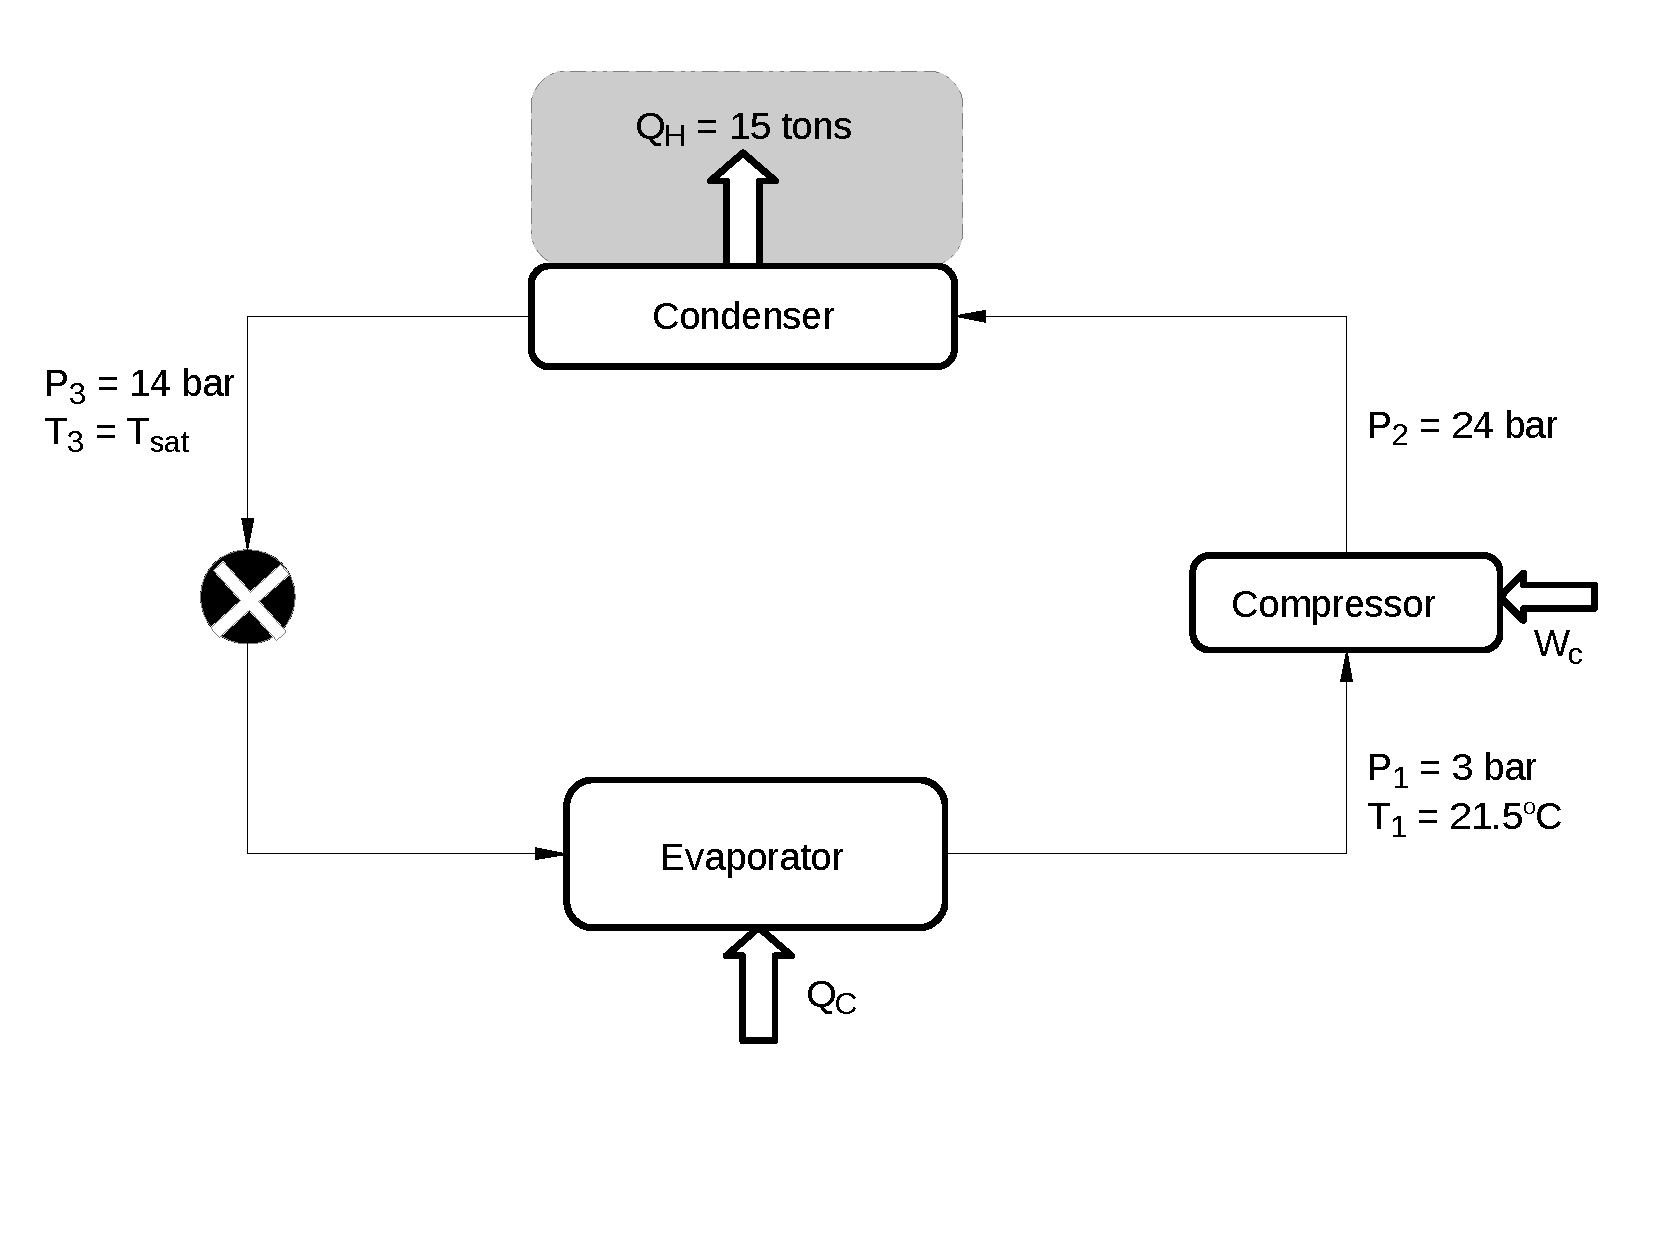
\includegraphics[width=12.0cm,height=9.0cm]{./Pics/Exam_Refrigeration14-15}
\end{center}
\vspace{-1.8cm}
\caption{Heat pump cycle.}\label{Exam01_Prob4}
\end{figure}
\begin{enumerate}[(i)]
 \item Specific enthalpies and entropies, h$_{i}$, s$_{i}$ with $i=\left\{1,2,3,4\right\}$;~\marks{8}
\solution{Calculating all properties:
\begin{description}
\item[1:] At P$_{1}$ =  3 bar and T$_{1}$= 21.5$^{\circ}$C $\rightarrow$  T$_{1}$ $>$ T$_{sat}$ (=-14.66$^{\circ}$C), thus the fluid is superheated vapour with \\
${\bf h_{1} = 268.88\text{ kJ.kg}^{-1}}$~\solmarks{1/8} and \\
${\bf s_{1} = 1.03915\text{ kJ.(kg.K)}^{-1}}$.~\solmarks{1/8}
\item[2:] The fluid undertakes an isentropic compression to P$_{2}$ = 24 bar, with \\
${\bf s_{2}=s_{1}}$ {\bf =1.03915  kJ.(kg.K)$^{-1}$}.~\solmarks{1/8} 
$s_{2} > s_{g}\left(P_{2}=24\text{ bar}\right)$, therefore the fluid is superheated vapour with $T_{2} = 131.41^{\circ}C$ and \\
${\bf h_{2} = 332.50\text{ kJ.kg}^{-1}}$.~\solmarks{1/8}
\item[3:] P$_{3}$ = 24 bar and T$_{3}$=T$_{sat}\left(P_{3}\right)$=59.46$^{\circ}$C, with \\
${\bf h_{3} = 121.56\text{ kJ.kg}^{-1}}$~\solmarks{1/8} and \\
${\bf s_{3} = 0.4241\text{ kJ.(kg.K)}^{-1}}$.~\solmarks{1/8}
\item[4:] Isenthalpic expansion to P$_{4}$=P$_{1}$ = 3 bar and \\
${\bf h_{4} = 121.56 \text{ kJ.kg}^{-1}}$~\solmarks{1/8} and \\
In order to calculate the entropy, we need first to calculate the quality of the vapour:
\begin{displaymath}
x_{4} = \frc{h_{4}-h_{f}}{h_{g}-h_{f}} = 0.4321
\end{displaymath}
and~\solmarks{1/8}
\begin{displaymath}
x_{4} = \frc{s_{4}-s_{f}}{s_{g}-s_{f}} = 0.4321 \Longrightarrow {\bf s_{4}=0.4755\text{ kJ.(kg.K)}^{-1}}.
\end{displaymath}
\end{description}
}
%

\item Mass flow rate $\left(\text{in kg.s}^{-1}\right)$ of the R-22 refrigerant fluid;~\marks{3}
\solution{Energy balance across the condenser with $Q_{H}$ = 15 tons = 52.5 kJ.s$^{-1}$:~\solmarks{3/3}
\begin{displaymath}
Q_{H} = \dot{m}_{R}\left(h_{3}-h_{2}\right)\;\; \Longrightarrow \;\; {\bf \dot{m}_{R} = 0.2499 \text{ kg.s}^{-1}}
\end{displaymath}
}
%

\item Compressor power $\left(W_{C}\right)$ and heat supplied $\left(Q_{C}\right)$ by the evaporator (in kW);~\marks{4}
\solution{Energy balance across the compressor:~\solmarks{2/4}
\begin{displaymath}
{\bf W_{C} =} \dot{m}_{R}\left(h_{2}-h_{1}\right) = {\bf 15.84 kW}.
\end{displaymath}
Energy balance across the evaporator:~\solmarks{2/4}
\begin{displaymath}
{\bf Q_{C} =} \dot{m}_{R}\left(h_{1}-h_{4}\right) = {\bf 36.67 kW}.
\end{displaymath}
}
%
\item Sketch the $Ts$ (temperature $\times$ specific entropy) and $Ph$ (pressure $\times$ specific enthalpy) diagrams of the cycle indicating all stages, isotherms and isobars.~\marks{5}
\solution{$Ts$ diagram:~\solmarks{2.5/5}
\begin{center}
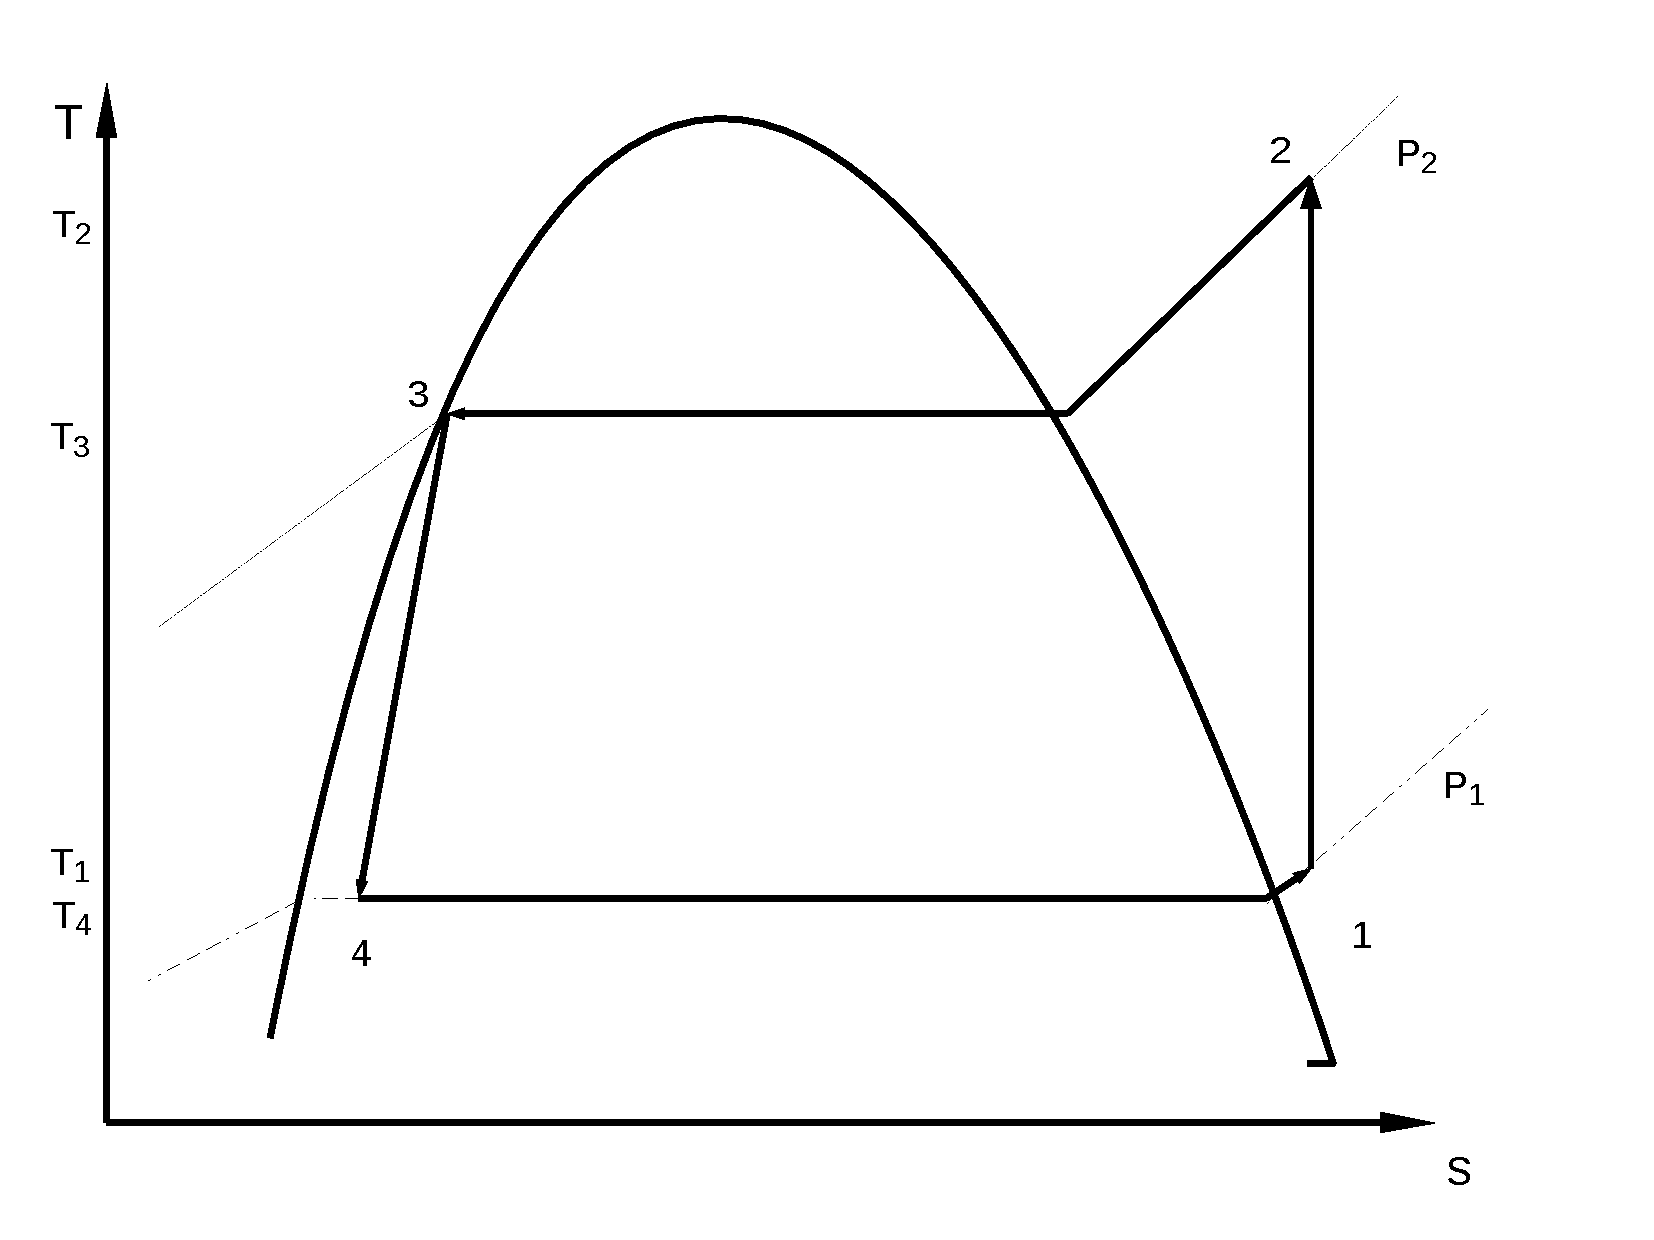
\includegraphics[width=8.0cm,height=8.0cm]{./Pics/Exam_TS_Refrig} 
\end{center}
$Ph$ diagram:~\solmarks{2.5/5}
\begin{center} 
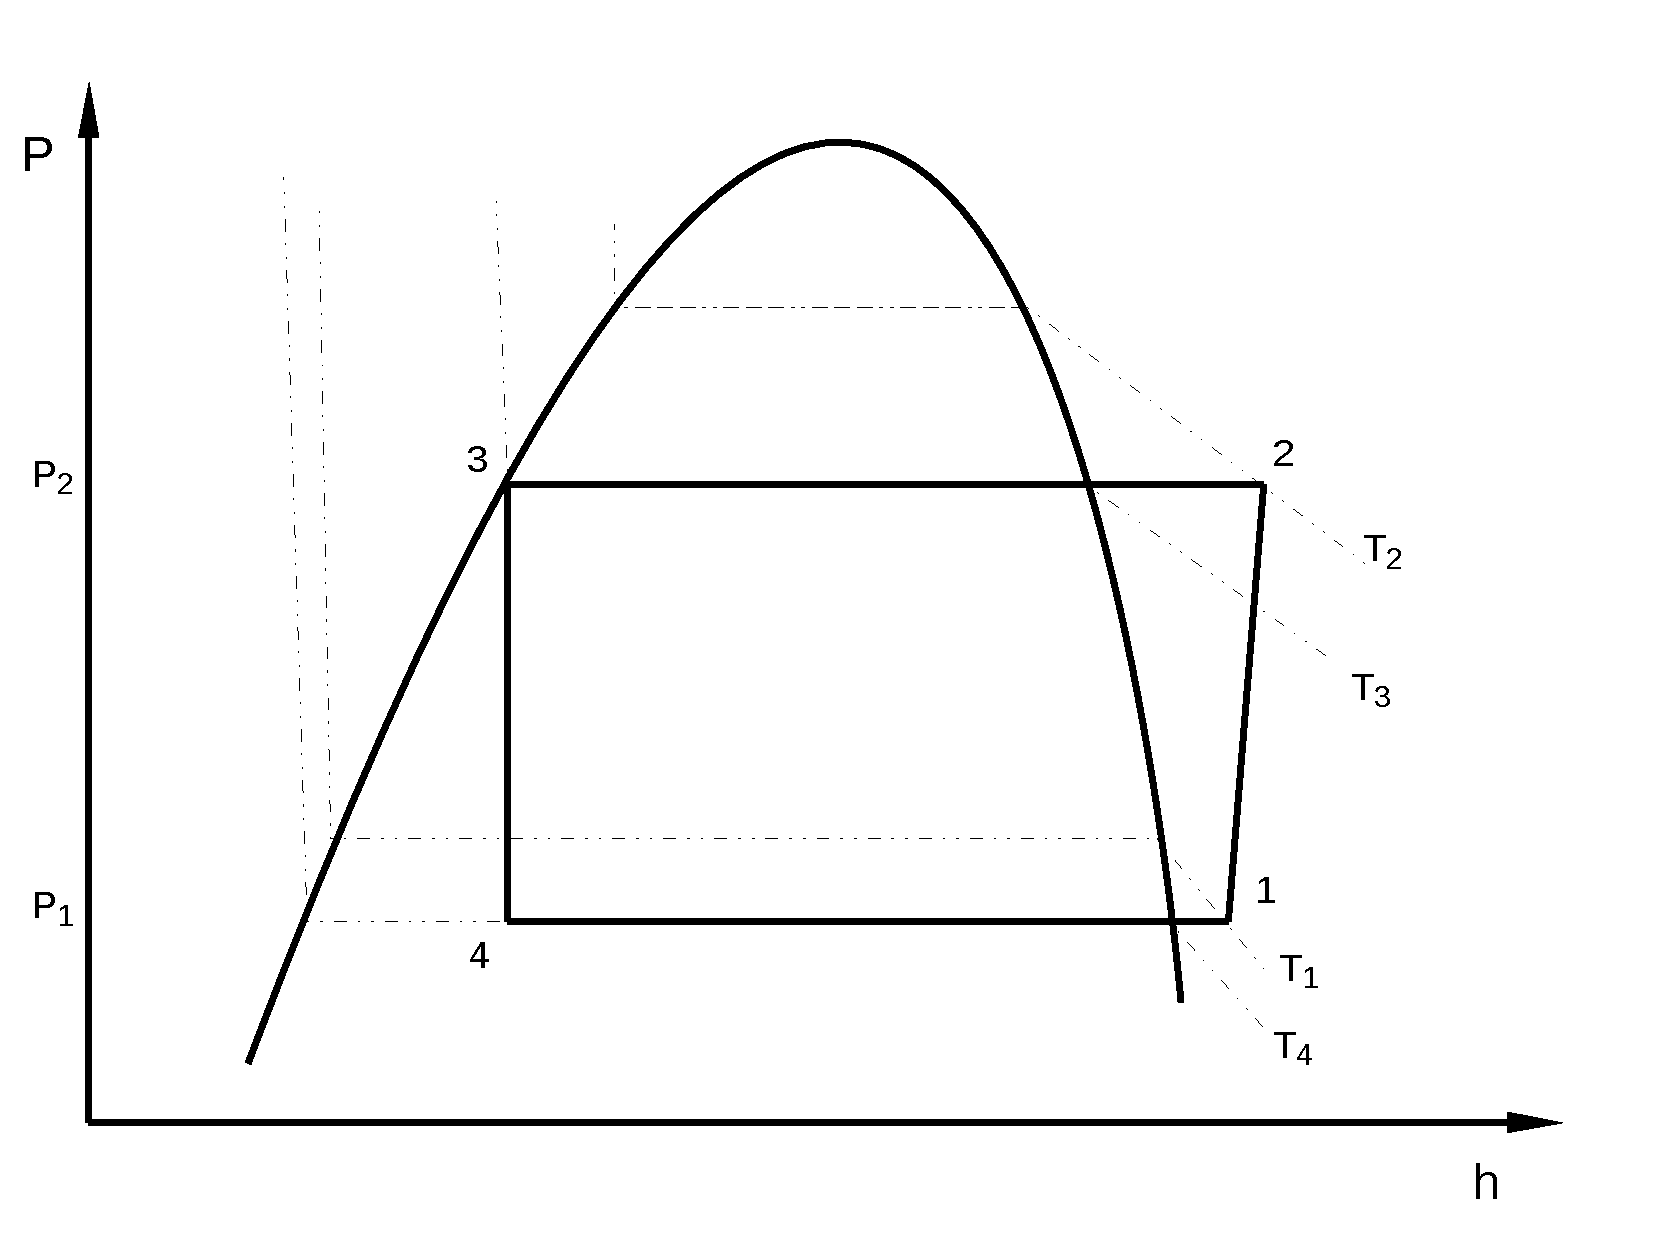
\includegraphics[width=8.0cm,height=8.0cm]{./Pics/Exam_PH_Refrig}
\end{center}
}
%%
\end{enumerate}
\end{question}

\clearpage

%%% 
%%% QUESTION (Saphiro 9.41 and 9.28)
%%%
\begin{question}
\begin{enumerate}[(a)]
\item In an ideal air-standard Brayton cycle, air enters the compressor at 1 bar and 300 K, with a mass flow rate of 6 kg.s$^{-1}$. The compressor ratio is 10, and the turbine inlet temperature is 1400 K. 
\begin{enumerate}[(i)]
\item Sketch the schematics of the cycle, $Ts$ (temperature $\times$ specific entropy) and $Pv$ (pressure $\times$ specific volume) diagrams. Indicate the numbering of each stage as used in your calculations;~\marks{3}
\solution{\solmarks{3/3}
    \begin{center}
      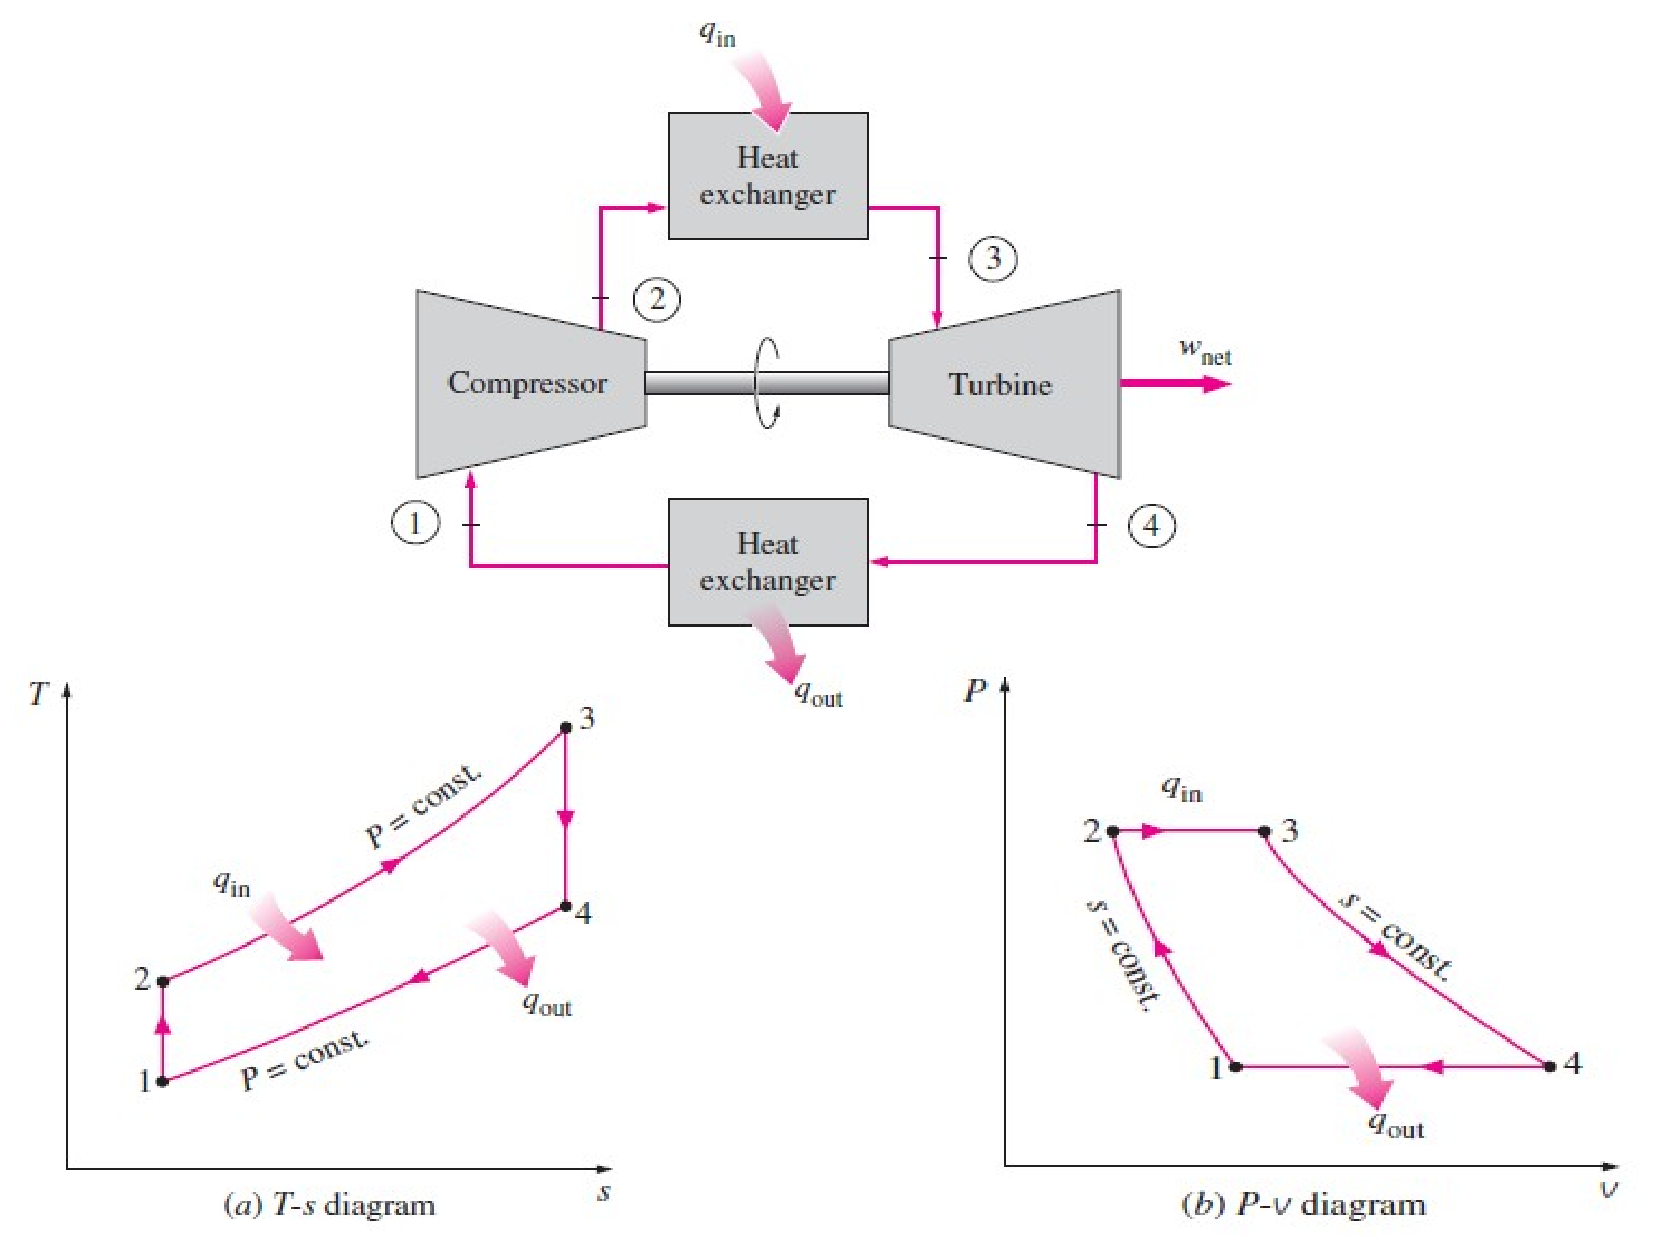
\includegraphics[height=7.cm,width=8.5cm,clip]{./Pics/Brayton_cycle1}
    \end{center}
}
\item Calculate the net power in MW;~\marks{4}
\solution{Given P$_{1}$ = 1 bar, T$_{1}$ = 300 K, T$_{3}$ = 1400 K, r$_{P}=\left(\frc{P_{2}}{P_{1}}\right)$ = 10 and $\dot{m}$ = 6 kg.s$^{-1}$, the net power $\left(\mathcal{P}_{\text{net}}\right)$ can be expressed as:
\begin{eqnarray}
\mathcal{P}_{\text{net}} &=& \text{Power produced by the Turbine} - \text{Power consumed by the Compressor} \nonumber \\
                       &=& \left|\dot{W}_{T}+\dot{W}_{C}\right| = \dot{m}C_{p}\left|\left(T_{4}-T_{3}\right) + \left(T_{2}-T_{1}\right)\right|. \nonumber
\end{eqnarray}
T$_{2}$ and T$_{4}$ can be calculated through:
\begin{description}
\item[1-2:] Isentropic compression:~\solmarks{1/4}
\begin{displaymath}
  T_{1}P_{1}^{\frac{1-\gamma}{\gamma}} = T_{2}P_{2}^{\frac{1-\gamma}{\gamma}}\;\;\rightarrow\;\;{\bf T_{2}= 579.21\text{ K}}
\end{displaymath}
\item[3-4:] Isentropic expansion:~\solmarks{1/4}
\begin{displaymath}
  T_{3}P_{3}^{\frac{1-\gamma}{\gamma}} = T_{4}P_{4}^{\frac{1-\gamma}{\gamma}}\;\;\rightarrow\;\;{\bf T_{4}= 725.13\text{ K}}
\end{displaymath}
\end{description}
Thus, {\bf $\mathcal{P}_{\text{net}}$= 2385.83 kJ.s$^{-1}$ = 2.38 MW}.~\solmarks{2/4}
}
\item Calculate the efficiency of the cycle;~\marks{3}
\solution{The efficiency is given by
\begin{displaymath}
\eta_{\text{Brayton}} = \frc{\text{Heat Supplied}-\text{Heat Rejected}}{\text{Heat Supplied}} =\frc{\dot{Q}_{in}-\dot{Q}_{out}}{\dot{Q}_{in}}
\end{displaymath}
where heat supplied is:~\solmarks{1/3}
\begin{displaymath}
{\bf \dot{Q}_{in}} = \dot{m}\left(h_{3}-h_{2}\right) = \dot{m}C_{p}\left(T_{3}-T_{2}\right) = {\bf 4949.36 \text{ kJ.s}^{-1}} 
\end{displaymath}
where heat rejected is:~\solmarks{1/3}
\begin{displaymath}
{\bf \dot{Q}_{out}} = \dot{m}\left(h_{1}-h_{4}\right) = \dot{m}C_{p}\left(T_{1}-T_{4}\right) = {\bf -2563.53 \text{ kJ.s}^{-1}} 
\end{displaymath}
The resulting efficiency is {\bf 48.20$\%$}.~\solmarks{1/3}
}
\end{enumerate}
%

\item The displacement volume of an internal combustion engine is 6400 cm$^{-3}$. Each cylinder in the engine operates as an air-standard Diesel cycle with cut-off ratio of 2.4. In the beginning of the compression, the conditions are: P$_{1}$ = 0.90 bar, T$_{1}$ = 27$^{\circ}$C and V$_{1}$ = 6.8$\times$10$^{-3}$ m$^{3}$.
\begin{enumerate}[(i)]
\item Determine V$_{2}$, V$_{3}$ $\left(\text{in m}^{3}\right)$, P$_{2}$ and P$_{4}$ (in bar);~\marks{4}
\solution{ Given:
\begin{itemize}
\item V$_{1}$ = 6.8$\times$10$^{-3}$ m$^{3}$
\item V$_{1}$-V$_{2}$ = 6.4$\times$10$^{-3}$ m$^{3}$ $\rightarrow$ {\bf V$_{2}$ = 0.4$\times$10$^{-3}$}~\solmarks{1/4} m$^{3}$ and $r=\frc{V_{1}}{V_{2}}$=17
\item $\rho$ = $\frc{\text{V}_{3}}{\text{V}_{2}}$= 2.4 
\item P$_{1}$ = 0.90 bar and T$_{1}$ = 300.15 K
\end{itemize}
\begin{description}
\item[1-2:] isentropic compression -- calculating P$_{2}$=P$_{3}$:~\solmarks{1/4}
\begin{displaymath}
P_{1}V_{1}^{\gamma} = P_{2}V_{2}^{\gamma}\;\rightarrow \;\; {\bf P_{2}=47.52\text{ bar }} =P_{3}
\end{displaymath}
now calculating T$_{2}$:
\begin{displaymath}
T_{1}V_{1}^{\gamma-1} = T_{2}V_{2}^{\gamma-1}\;\;\rightarrow\;\; T_{2}= 932.22\text{ K}
\end{displaymath}
\item[2-3:] expansion at constant volume -- with the cut-off ratio $\rho=\frc{V_{3}}{V_{2}}=2.4$ $\rightarrow$ {\bf V$_{3}$ = 0.96$\times$10$^{-3}$ m$^{3}$}~\solmarks{1/4}
\begin{displaymath}
\frc{T_{2}}{V_{2}} = \frc{T_{3}}{V_{3}} \;\;\rightarrow\;\;T_{3}=2237.33\text{ K}
\end{displaymath}
\item[3-4:] isentropic expansion -- calculating P$_{4}$ and T$_{4}$:~\solmarks{1/4}
\begin{eqnarray}
P_{3}V_{3}^{\gamma} = P_{4}V_{4}^{\gamma}\rightarrow {\bf P_{4}}=P_{3}\left(\frc{V_{3}}{V_{4}}\right)^{\gamma} = P_{3}\left(\frc{\rho}{r}\right)^{\gamma} = {\bf 3.07\text{ bar }}
\end{eqnarray}
\end{description}
}
%
\item Calculate the thermal efficiency of the cycle;~\marks{3}
\solution{ Thermal efficiency is defined as~\solmarks{3/3}
\begin{eqnarray}
{\bf \eta} &=& \frc{\text{Heat Supplied} - \text{Heat Rejected}}{\text{Heat Supplied}} = \frc{C_{p}\left(T_{3}-T_{2}\right)-C_{v}\left(T_{4}-T_{1}\right)}{C_{p}\left(T_{3}-T_{2}\right)} \nonumber \\
           &=& 1-\frc{T_{4}-T_{1}}{\gamma\left(T_{3}-T_{2}\right)} ={\bf 0.6047}\nonumber
\end{eqnarray}
}
\item Calculate the net work (in kJ) using the following expression:~\marks{3}
\begin{displaymath}
W_{\text{net}} = \frc{P_{1}V_{1} r^{\gamma-1}\left[\gamma\left(\rho-1\right)-r^{1-\gamma}\left(\rho^{\gamma}-1\right)\right]}{\gamma-1},
\end{displaymath}
where $r$ and $\rho$ are the compression and cut-off ratios, respectively. 
\solution{ With $r=17$ and $\rho=2.4$,\solmarks{3/3}
\begin{eqnarray}
{\bf W_{\text{net}}} &=& \frc{P_{1}V_{1} r^{\gamma-1}\left[\gamma\left(\rho-1\right)-r^{1-\gamma}\left(\rho^{\gamma}-1\right)\right]}{\gamma-1} \nonumber \\
                   &=& 0.05632\text{ bar.m}^{3} = {\bf 5.63 \text{ kJ}}  \nonumber
\end{eqnarray}

}

\end{enumerate}
%
\end{enumerate}

Assume that air behaves as an ideal gas with the following properties: MW = 29 g.mol$^{-1}$, C$_{p}$ = 1.005 kJ.(kg.K)$^{-1}$ and C$_{v}$ = 0.718 kJ.(kg.K)$^{-1}$, where MW is the molar mass and C$_{p}$ and C$_{v}$ are the heat capacities at constant pressure and volume, respectively. Also, given the following relations for isentropic operations with $\gamma = \displaystyle\frac{C_{p}}{C_{v}}$:
\begin{displaymath}
TV^{\gamma-1}=\text{constant},\;\; TP^{\frac{1-\gamma}{\gamma}}=\text{constant and }\;\; PV^{\gamma}=\text{constant} 
\end{displaymath}

\end{question}

\clearpage

%%% 
%%% QUESTION (Jeff's mind)
%%%
\begin{question}
The ideal regenerative Rankine cycle (open feedwater heater, Fig.~\ref{exam2_Q3_rankinecycle}) shown below is operated with water-steam as working fluid to produce power $\left(W_{T}\right)$. Someproperties of the cycle are shown in Table~\ref{IRRC_Table} and the mass flow rate leaving the boiler is 1 kg.s$^{-1}$.
      \begin{figure}[h]
      \begin{center}
      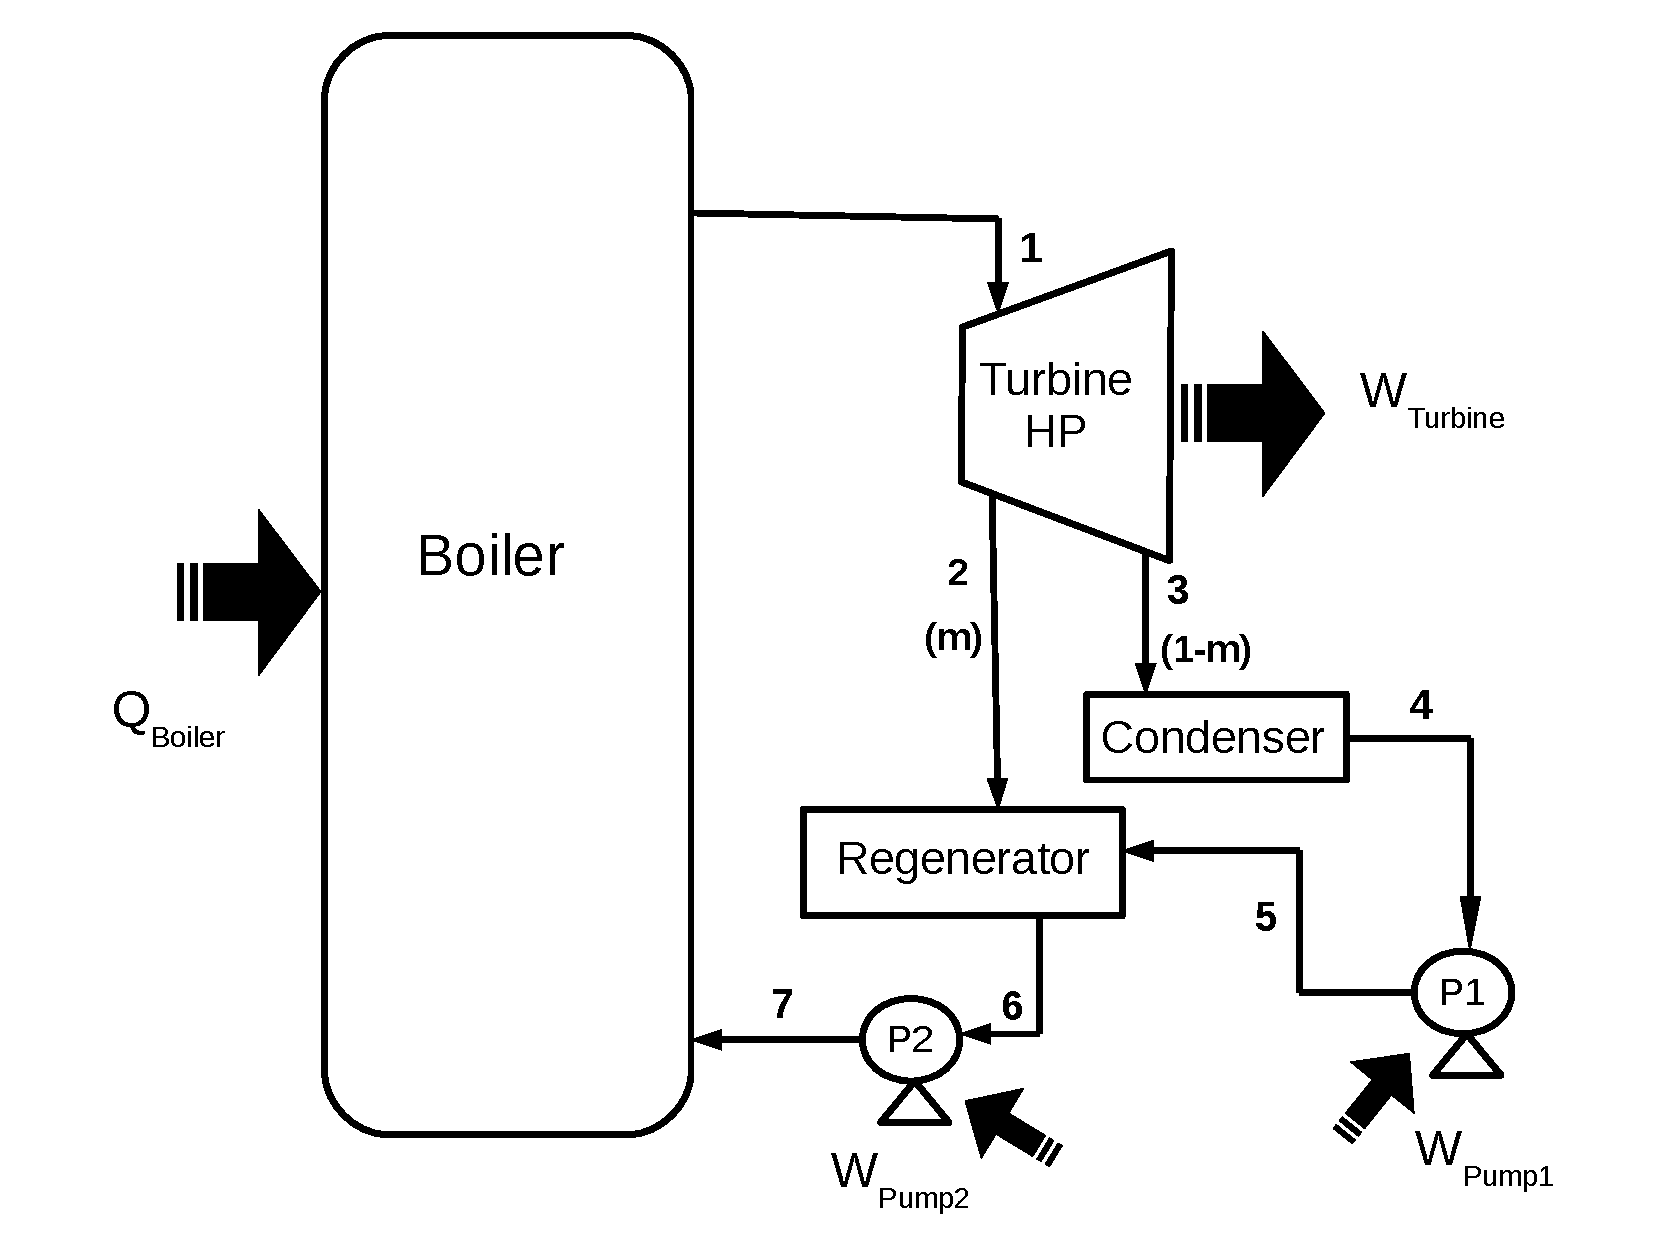
\includegraphics[width=10.cm,clip]{./Pics/Exam_Reheat_Regenerative2_Rankine_Cycle}
      \caption{Regenerative Rankine cycle.}
      \label{exam2_Q3_rankinecycle}
     \end{center} 
     \end{figure}
\begin{table}[b]
\begin{center}
\begin{tabular}{c | c c c c c c} 
\hline
{\bf Stage} & {\bf P}       & {\bf T}            &  {\bf State}  &  {\bf Quality}  & {\bf h}             & {\bf s}                  \\
            & {\bf (bar)}   & {\bf ($^{\circ}$C)} &               &                 &{\bf (kJ.kg$^{-1}$)}  & {\bf (kJ.(kg.K)$^{-1}$)}  \\
\hline
1           &  200          & 480                &  {\bf (a)}    &   --            & {\bf (b)}           & {\bf (c)}                 \\
2           &  30           & {\bf (d)}          &  Wet vapour   & {\bf (e)}       & {\bf (f)}           & {\bf (g)}                \\
3           &  5            & --                 &  Wet vapour   & {\bf (h)}       & {\bf (i)}           & {\bf (j)}                \\
4           &  {\bf (k)}    &  --                &  {\bf (l)}    & --              &   --                &   --                      \\
5           &  30           &  --                &   --          &  --             & {\bf (m)}           &  --                       \\
6           &  30           &  --                &   --          &  --             & {\bf (n)}           &  --                       \\
7           &  {\bf (o)}    &  --                &   --          &  --             & {\bf (p)}           &  --                       \\
\hline
\end{tabular}
\end{center}
\caption{Conditions of the ideal regenerative Rankine cycle.}\label{IRRC_Table}
\end{table}
\begin{enumerate}[(a)]
\item Determine (a-p) in Table~\ref{IRRC_Table};~\marks{16}
\solution{\begin{description}
\item[Stage 1:] At P$_{1}$ = 200 bar and T$_{1}$ = 480$^{\circ}$C the fluid is {\bf superheated fluid (SHF)}~\solmarks{1/16} with:
\begin{itemize}
\item {\bf h$_{1}$ = 3170.8 kJ.kg$^{-1}$}~\solmarks{1/16} and
\item {\bf s$_{1}$ = 6.0518 kJ.(kg.K)$^{-1}$}~\solmarks{1/16}
\end{itemize}

\item[Stage 2:] At P$_{2}$ = 30 bar, the temperature of the wet vapour is the same as the saturated temperature, i.e., {\bf T$_{2}$} = T$_{\text{sat}}$ = {\bf 233.9$^{\circ}$C}~\solmarks{1/16}. The fluid suffered an isentropic expansion, i.e., {\bf s$_{2}$} = s$_{1}$ = {\bf 6.0518 kJ.(kg.K)$^{-1}$}.~\solmarks{1/16} 

We can calculate the quality of the vapour as,~\solmarks{1/16}
\begin{displaymath}
s_{2}=s_{f2}+x_{2}\left(s_{g2}-s_{f2}\right) \;\; \rightarrow {\bf x_{2} = 0.9618} 
\end{displaymath}
and the enthalpy~\solmarks{1/16}
\begin{displaymath}
h_{2}=h_{f2}+x_{2}\left(h_{g2}-h_{f2}\right) \;\; \rightarrow {\bf h_{2} = 2735.60\text{ kJ.kg}^{-1}} 
\end{displaymath}

\item[Stage 3:] At P$_{3}$ = 5 bar (and using the same procedure as in Stage 2):
\begin{itemize}
\item {\bf s$_{3}$} = s$_{1}$ = {\bf 6.0518 kJ.(kg.K)$^{-1}$}~\solmarks{1/16}
\item {\bf x$_{3}$ = 0.8449}~\solmarks{1/16}
\item {\bf h$_{3}$ = 2421.68 kJ.kg$^{-1}$}~\solmarks{1/16} 
\end{itemize}

\item[Stage 4:] Fluid leaving the condenser is {\bf saturated liquid (SL)}~\solmarks{1/16} with
\begin{itemize}
\item {\bf P$_{4}$} = P$_{3}$ = {\bf 5 bar}~\solmarks{1/16}
\item h$_{4}$ = h$_{f}$(P = 5 bar) =  640.23 kJ.kg$^{-1}$
\item v$_{4}$ = v$_{f}$(P = 5 bar) = 1.0926$\times$10$^{-3}$ m$^{3}$.kg$^{-1}$
\end{itemize}

\item[Stage 5:] Fluid is assumed incompressible with $dh = vdP$ and~\solmarks{1/16}
\begin{displaymath}
{\bf h_{5}} = h_{4} + v_{4}\left(P_{5}-P_{4}\right) = {\bf 642.96 \text{ kJ.kg}^{-1}}
\end{displaymath}

\item[Stage 6:]  Fluid leaving the regenerator is saturated liquid with
\begin{itemize}
\item {\bf h$_{6}$} = h$_{f}$(P = 30 bar) =  {\bf 1008.4 kJ.kg$^{-1}$}~\solmarks{1/16}
\item v$_{6}$ = v$_{f}$(P = 30 bar) = 1.2165$\times$10$^{-3}$ m$^{3}$.kg$^{-1}$
\end{itemize}


\item[Stage 7:]  Fluid is assumed incompressible with $dh = vdP$ with {\bf P$_{7}$=P$_{1}$= 200 bar}~\solmarks{1/16} and
\begin{displaymath}
{\bf h_{7}} = h_{6} + v_{6}\left(P_{7}-P_{6}\right) = {\bf 1029.08 \text{ kJ.kg}^{-1}}
\end{displaymath}~\solmarks{1/16}
\end{description}

\begin{center}
\begin{tabular}{c | c c c c c c} 
\hline
{\bf Stage} & {\bf P}       & {\bf T}            &  {\bf State}  &  {\bf Quality}  & {\bf h}             & {\bf s}                  \\
            & {\bf (bar)}   & {\bf ($^{\circ}$C)} &               &                 &{\bf (kJ.kg$^{-1}$)}  & {\bf (kJ.(kg.K)$^{-1}$)}  \\
\hline
1           &  200          & 480                &  {\bf (a) SHF}&   --            & {\bf (b) 3170.80}    & {\bf (c) 6.0518}         \\
2           &  30           & {\bf (d) 233.90}    &  Wet vapour   & {\bf (e) 0.9618}& {\bf (f) 2735.60}   & {\bf (g) 6.0518}         \\
3           &  5            & --                 &  Wet vapour   & {\bf (h) 0.8449}& {\bf (i) 2421.68}   & {\bf (j) 6.0518}          \\
4           &  {\bf (k) 5}  &  --                &  {\bf (l) SL} & --              &   --                &   --                      \\
5           &  30           &  --                &   --          &  --             & {\bf (m) 642.96}    &  --                       \\
6           &  30           &  --                &   --          &  --             & {\bf (n) 1008.40}    &  --                       \\
7           &  {\bf (o) 200}&  --                &   --          &  --             & {\bf (p) 1029.08}   &  --                       \\
\hline
\end{tabular}
\end{center}

}

\item Calculate the heat supplied by the boiler $\left(\text{Q}_{\text{Boiler}}\right)$, the power produced by the turbine $\left(\text{W}_{\text{Turbine}}\right)$ and the power required by the pumps $\left(\text{W}_{\text{Pump1}}\text{ and W}_{\text{Pump2}}\right)$. All these quantities in kW.~\marks{4}
\solution{ Before calculating the power and heat associated with the cycle, we first need to obtain the fraction {\it (m)} of water-steam that is driven to the regenerator. An energy balance around the regenerator leads to:
\begin{displaymath}
m h_{2} + (1-m)h_{5} = 1 \times h_{6} \;\;\rightarrow \;\; m = 0.1746 \text{ kg.s}^{-1}
\end{displaymath}
\begin{itemize}
\item ${\bf Q_{\text{Boiler}}} = m\left(h_{1}-h_{7}\right) = {\bf 2141.2\text{ kW}}$~\solmarks{1/4}
\item ${\bf T_{\text{Turbine}}} =(1-m)h_{3} + mh_{2} - h_{1} = {\bf -694.31\text{ kW}}$~\solmarks{1/4}
\item ${\bf W_{\text{Pump1}}} = (1-m)\left(h_{5}-h_{4}\right) = {\bf 0.48\text{ kW}}$~\solmarks{1/4}
\item ${\bf W_{\text{Pump2}}} = h_{7}-h_{6} = {\bf 20.68 \text{ kW}}$~\solmarks{1/4}
\end{itemize}


}
\end{enumerate}

To solve this problem, you should assume that the saturated liquid streams are incompressible, and therefore $dh = vdP$ (where $h$, $v$ and $P$ are specific enthalpy, volume and pressure, respectively). Quality of the vapour is expressed as
\begin{displaymath}
x_{j} = \frc{\Psi_{j}-\Psi_{f}}{\Psi_{g}-\Psi_{f}}\;\;\;\text{with }\Psi=\left\{h,s\right\},\text{ where } s \text{ is the specific entropy.}
\end{displaymath}


\end{question}

\clearpage


%%%%%%%%%%%%%%%%%%%%%%%%%
%%% Question 04       %%%
%%%%%%%%%%%%%%%%%%%%%%%%%
\begin{question} 


\begin{enumerate}[(a)]
\item Gas flows along a pipe of constant cross section $A$ $\left(\text{m}^2\right)$, in the direction of increasing $x$. By considering the rate of change of the mass of gas within a small section of pipe and the gas mass fluxes into and out of this section of pipe, show that
\begin{align*}
 \fracp{\rho}{t} + \fracp{}{x}\left(\rho u\right) = 0.
\end{align*}
Here the gas velocity $u$ and the gas density $\rho$ are functions of $x$ and time $t$. \marks{5} \\
\solution{The total mass contained in a section of pipe of length $\Delta x$ is $\rho A \Delta x$.  \solmarks{1/5}

The rate of change of mass in this section of pipe equals the mass flux entering the pipe $\rho u A$, minus the mass flux leaving the other end of the pipe section
\begin{align*}
 \rho u A + \Delta x \fracp{}{x}\left(\rho u A\right).
\end{align*}
[Obtained via a linearized Taylor expansion.] \solmarks{2/5}

Hence mass conservation implies
\begin{align*}
 \fracp{}{t}\left(\rho A \Delta x\right) = \rho u A - \rho u A - \Delta x \fracp{}{x}\left(\rho u A\right).
\end{align*}
and hence dividing by $A \Delta x$ and rearranging gives the result. \solmarks{2/5}
}

%%%%%%%%%%%
\item Explain what is meant by a steady flow and show that for steady flow in a pipe of constant cross section
\begin{align*}
 \frac{1}{\rho} \fracd{\rho}{x} + \frac{1}{u} \fracd{u}{x} = 0.
\end{align*} \marks{4}
\solution{The flow is steady if the density, velocity and cross section depend only on $x$ and not time $t$. In this case the result from (a) gives
\begin{align*}
 \fracd{}{x}\left(\rho u\right) = 0.
\end{align*}~\solmarks{2/4}

Therefore via the chain rule
\begin{align*}
 \rho \fracd{u}{x} + u \fracd{\rho}{x} = 0.
\end{align*}
Finally dividing by $\rho u$ gives the required result.\solmarks{2/4}}

%%%%%%%%%%%
\item The beginning of a pipe of constant cross section is located at $x=0$, where the gas velocity into the pipe $u=4$\,m/s. If the gas density profile along the pipe is 
\begin{align*}
 \rho\br{x} = (1 - 0.02x)\,\mbox{kg/m}^3,
\end{align*}
then determine the gas velocity at $x=2$ m. \marks{7}
\solution{Substituting in the formula from the previous section
\begin{align*}
 \frac{1}{u} \fracd{u}{x} = -\frac{1}{\rho} \fracd{\rho}{x} = -\frac{-0.02}{1 - 0.02x} = \frac{0.02}{1 - 0.02x}.
\end{align*}\solmarks{2/7}

Integrating with respect to $x$
\begin{align*}
 \int_4^u \frac{\d{\tilde{u}}}{\tilde{u}} = \int_0^2 \frac{0.02 \,\d{x}}{1 - 0.02x}.
\end{align*} \solmarks{2/7}

Hence
\begin{align*}
 \left[\log\br{\tilde{u}}\right]_4^u = \left[-\log\br{1 - 0.02x}\right]_0^2,
\end{align*}
\begin{align*}
 \log\br{\frac{u}{4}} = -\log\br{1 - 0.04} + \log\br{1} = \log\br{\frac{1}{0.96}},
\end{align*}\solmarks{1/7}

Exponentiating both sides gives $u = 4/0.96 = 4.1667$\,m/s. \solmarks{2/7}}

%%%%%%%%%%%
\item Gas flows into and out of a steady flow device at a total of three different locations. At the first location gas with density $\rho=1.4$\,kg/m$^3$ flows into the device with velocity $u=4$\,m/s  through a pipe of cross section $A=0.2$\,m$^2$. At the second location gas with density $0.9$\,kg/m$^3$ flows out of the device with velocity $u=5$\,m/s through a pipe of cross section $A=0.4$\,m$^2$. At the third location, determine whether gas is flowing into or out of the device. \marks{4}
\solution{The mass flux into the device at the first location is $\rho u A = 1.4\times 4 \times 0.2 = 1.12$\,kg/s. \solmarks{1/4}

The mass flux out of the device at the second location is $\rho u A = 0.9\times 5 \times 0.4 = 1.8$\,kg/s. \solmarks{1/4} 

More gas is flowing out of the device at the second location than is flowing into the device at the first location, and therefore there must be an additional mass flux into the device at the third location. \solmarks{2/4}
}
\end{enumerate}
\end{question}

\clearpage

%%%%%%%%%%%%%%%%%%%%%%%%%
%%% Question 05       %%%
%%%%%%%%%%%%%%%%%%%%%%%%%
\begin{question} 
\begin{enumerate}[(a)]
%%%%%%%%%%%%%%%%%%%%%%%%%%
\item Air in an air-conditioning system is mixed adiabatically with air from outside in a steady process. If the inlets to the mixing chamber are labelled 1 and 2, and the outlet is labelled 3, then state equations that correspond to the mass conservation of dry air, the mass conservation of water vapour and the conservation of energy in this situation. Hence, show that
\begin{align*}
 \frac{\dot{m}_{a_1}}{\dot{m}_{a_2}} = \frac{h_3 - h_2}{h_1 - h_3} = \frac{\omega_3 - \omega_2}{\omega_1 - \omega_3},
\end{align*}
where $\dot{m}_a$ is a mass flux of dry air, $h$ is a specific enthalpy and $\omega$ is a specific humidity.\marks{8}
\solution{
In the mixing section
\begin{align*}
\mbox{\textit{Conservation of dry air:}} & & \dot{m}_{a_1} + \dot{m}_{a_2} = \dot{m}_{a_3}, \\
\mbox{\textit{Conservation of water vapour:}} & & \dot{m}_{a_1} \omega_1 + \dot{m}_{a_2} \omega_2 = \dot{m}_{a_3} \omega_3, \\
\mbox{\textit{Conservation of energy:}} & & \dot{m}_{a_1} h_1 + \dot{m}_{a_2} h_2 = \dot{m}_{a_3} h_3.
\end{align*}~\solmarks{3/8}

Using the dry air mass conservation equation to eliminate $\dot{m}_{a_3}$ from the other two expressions, gives
\begin{align*}
 \dot{m}_{a_1} \omega_1 + \dot{m}_{a_2} \omega_2 =& \left(\dot{m}_{a_1} + \dot{m}_{a_2}\right) \omega_3, \\
 \dot{m}_{a_1} h_1 + \dot{m}_{a_2} h_2 =& \left(\dot{m}_{a_1} + \dot{m}_{a_2}\right) h_3.
\end{align*}~\solmarks{2/8}

Collecting all the terms involving $\dot{m}_{a_2}$ on the left-hand side and all the terms involving $\dot{m}_{a_3}$ on the right-hand side gives
\begin{align*}
 \dot{m}_{a_2} \omega_2 - \dot{m}_{a_2} \omega_3 =& \dot{m}_{a_1} \omega_3 - \dot{m}_{a_1} \omega_1, \\
 \dot{m}_{a_2} h_2 - \dot{m}_{a_1} h_3 =& \dot{m}_{a_2} h_3 - \dot{m}_{a_1} h_1.
\end{align*}~\solmarks{1/8}

Rearranging
\begin{align*}
 \dot{m}_{a_2} \left(\omega_3 - \omega_2\right) =& \dot{m}_{a_1} \left(\omega_1 - \omega_3\right), \\
 \dot{m}_{a_2} \left(h_3 - h_2\right) =& \dot{m}_{a_2} \left(h_1 - h_3\right).
\end{align*}~\solmarks{1/8}

Finally
\begin{align*}
 \frac{\dot{m}_{a_1}}{\dot{m}_{a_2}} = \frac{\omega_3 - \omega_2}{\omega_1 - \omega_3}, \quad \mbox{and} \quad \frac{\dot{m}_{a_2}}{\dot{m}_{a_2}} =& \frac{h_3 - h_2}{h_1 - h_3},
\end{align*}
which gives the necessary result.\solmarks{1/8}
}

%%%%%%%%%%%%%%%%%%%%%%%%%%
\item Inlet 1 draws saturated air from the cooling section of the air conditioning system at a dry bulb temperature of $5^\circ$C. Inlet 2 takes air from outside with a specific humidity of 0.025\,kg water/kg dry air. The dry bulb temperature of the resulting mixture is $20^\circ$C. If liquid water is not produced in the mixing chamber, then determine the minimum dry bulb temperature of air entering the system through inlet 2. \marks{4}
\solution{Liquid water is not produced in the mixing chamber, so the relative humidity of the mixed gas is equal or less than 100\%. \solmarks{1/4}

On the psychrometric chart the line linking ($T_1=5^\circ$C, $\phi_1=100\%$) and ($T_3=20^\circ$C, $\phi_3=100\%$) intersects the line $\omega_2=0.025\,$kg water/kg dry air when $T_2 = 36^\circ$C. \solmarks{1/4}

Any temperature $T > T_3$ will not produce liquid water in the mixing chamber, so the minimum temperature in inlet 2 is $36^\circ$C. \solmarks{2/4}
}

%%%%%%%%%%%%%%%%%%%%%%%%%%
\item Additionally, it is known that the gas mass flux in inlet 2 is twice the gas mass flux in inlet 1.
\begin{enumerate}[(i)]
\item Determine the specific and relative humidity of the mixture; \marks{6}
\solution{From the psychrometric chart the specific humidity of inlet 1 is $\omega_1 = 0.0055$\,kg water/kg dry air.

Rearrange equation part (a) to give
\begin{align*}
 \left(1 + \frac{\dot{m}_{a_1}}{\dot{m}_{a_2}}\right)\omega_3 = \omega_1 + \frac{\dot{m}_{a_1}}{\dot{m}_{a_2}} \omega_2.
\end{align*}\solmarks{2/6}

Therefore
\begin{align*}
 \omega_3 = \frac{0.0055 + \left(0.5\times0.025\right)}{1 + 0.5} = 0.012 \mbox{kg water/kg dry air}.
\end{align*}\solmarks{2/6}

From the psychrometric chart, the relative humidity of the mixture is 82\%. \solmarks{2/6}
}

\item Determine the dry bulb temperature at inlet 2. \marks{2}
\solution{On the psychrometric chart the line linking ($T_1=5^\circ$C, $\phi_1=100\%$) and ($T_3=5^\circ$C, $\omega_3=0.012$\,kg water/kg dry air) intersects the line $\omega_2=0.025\,$kg water/kg dry air when $T_2 = 48.5^\circ$C. Therefore the temperature of the gas in inlet 2 is $48.5^\circ$C. \solmarks{2/2}}
\end{enumerate}
\end{enumerate}
\end{question}


\vfill


\paperend

%\begin{comment}
{
  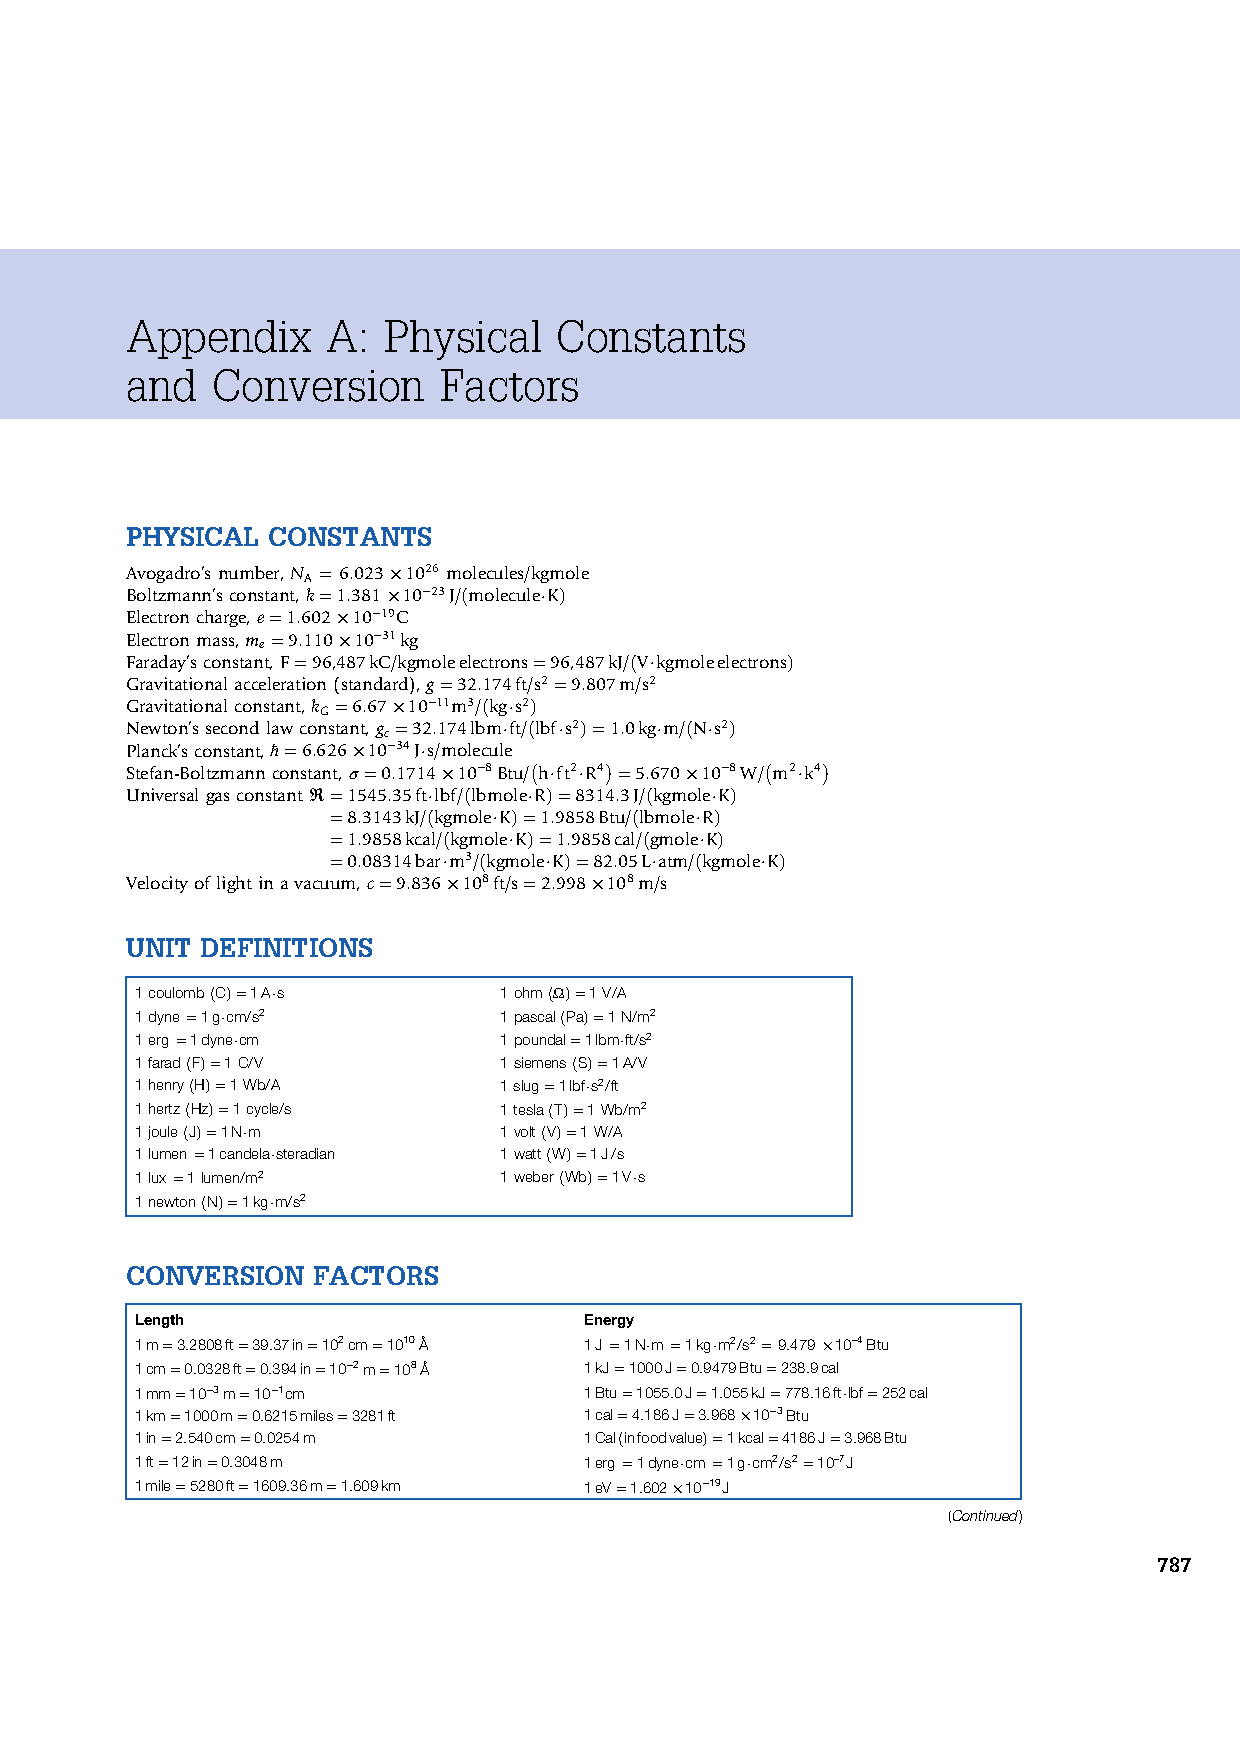
\includepdf[pages=-,fitpaper]{./Pics/UnitConversion}
  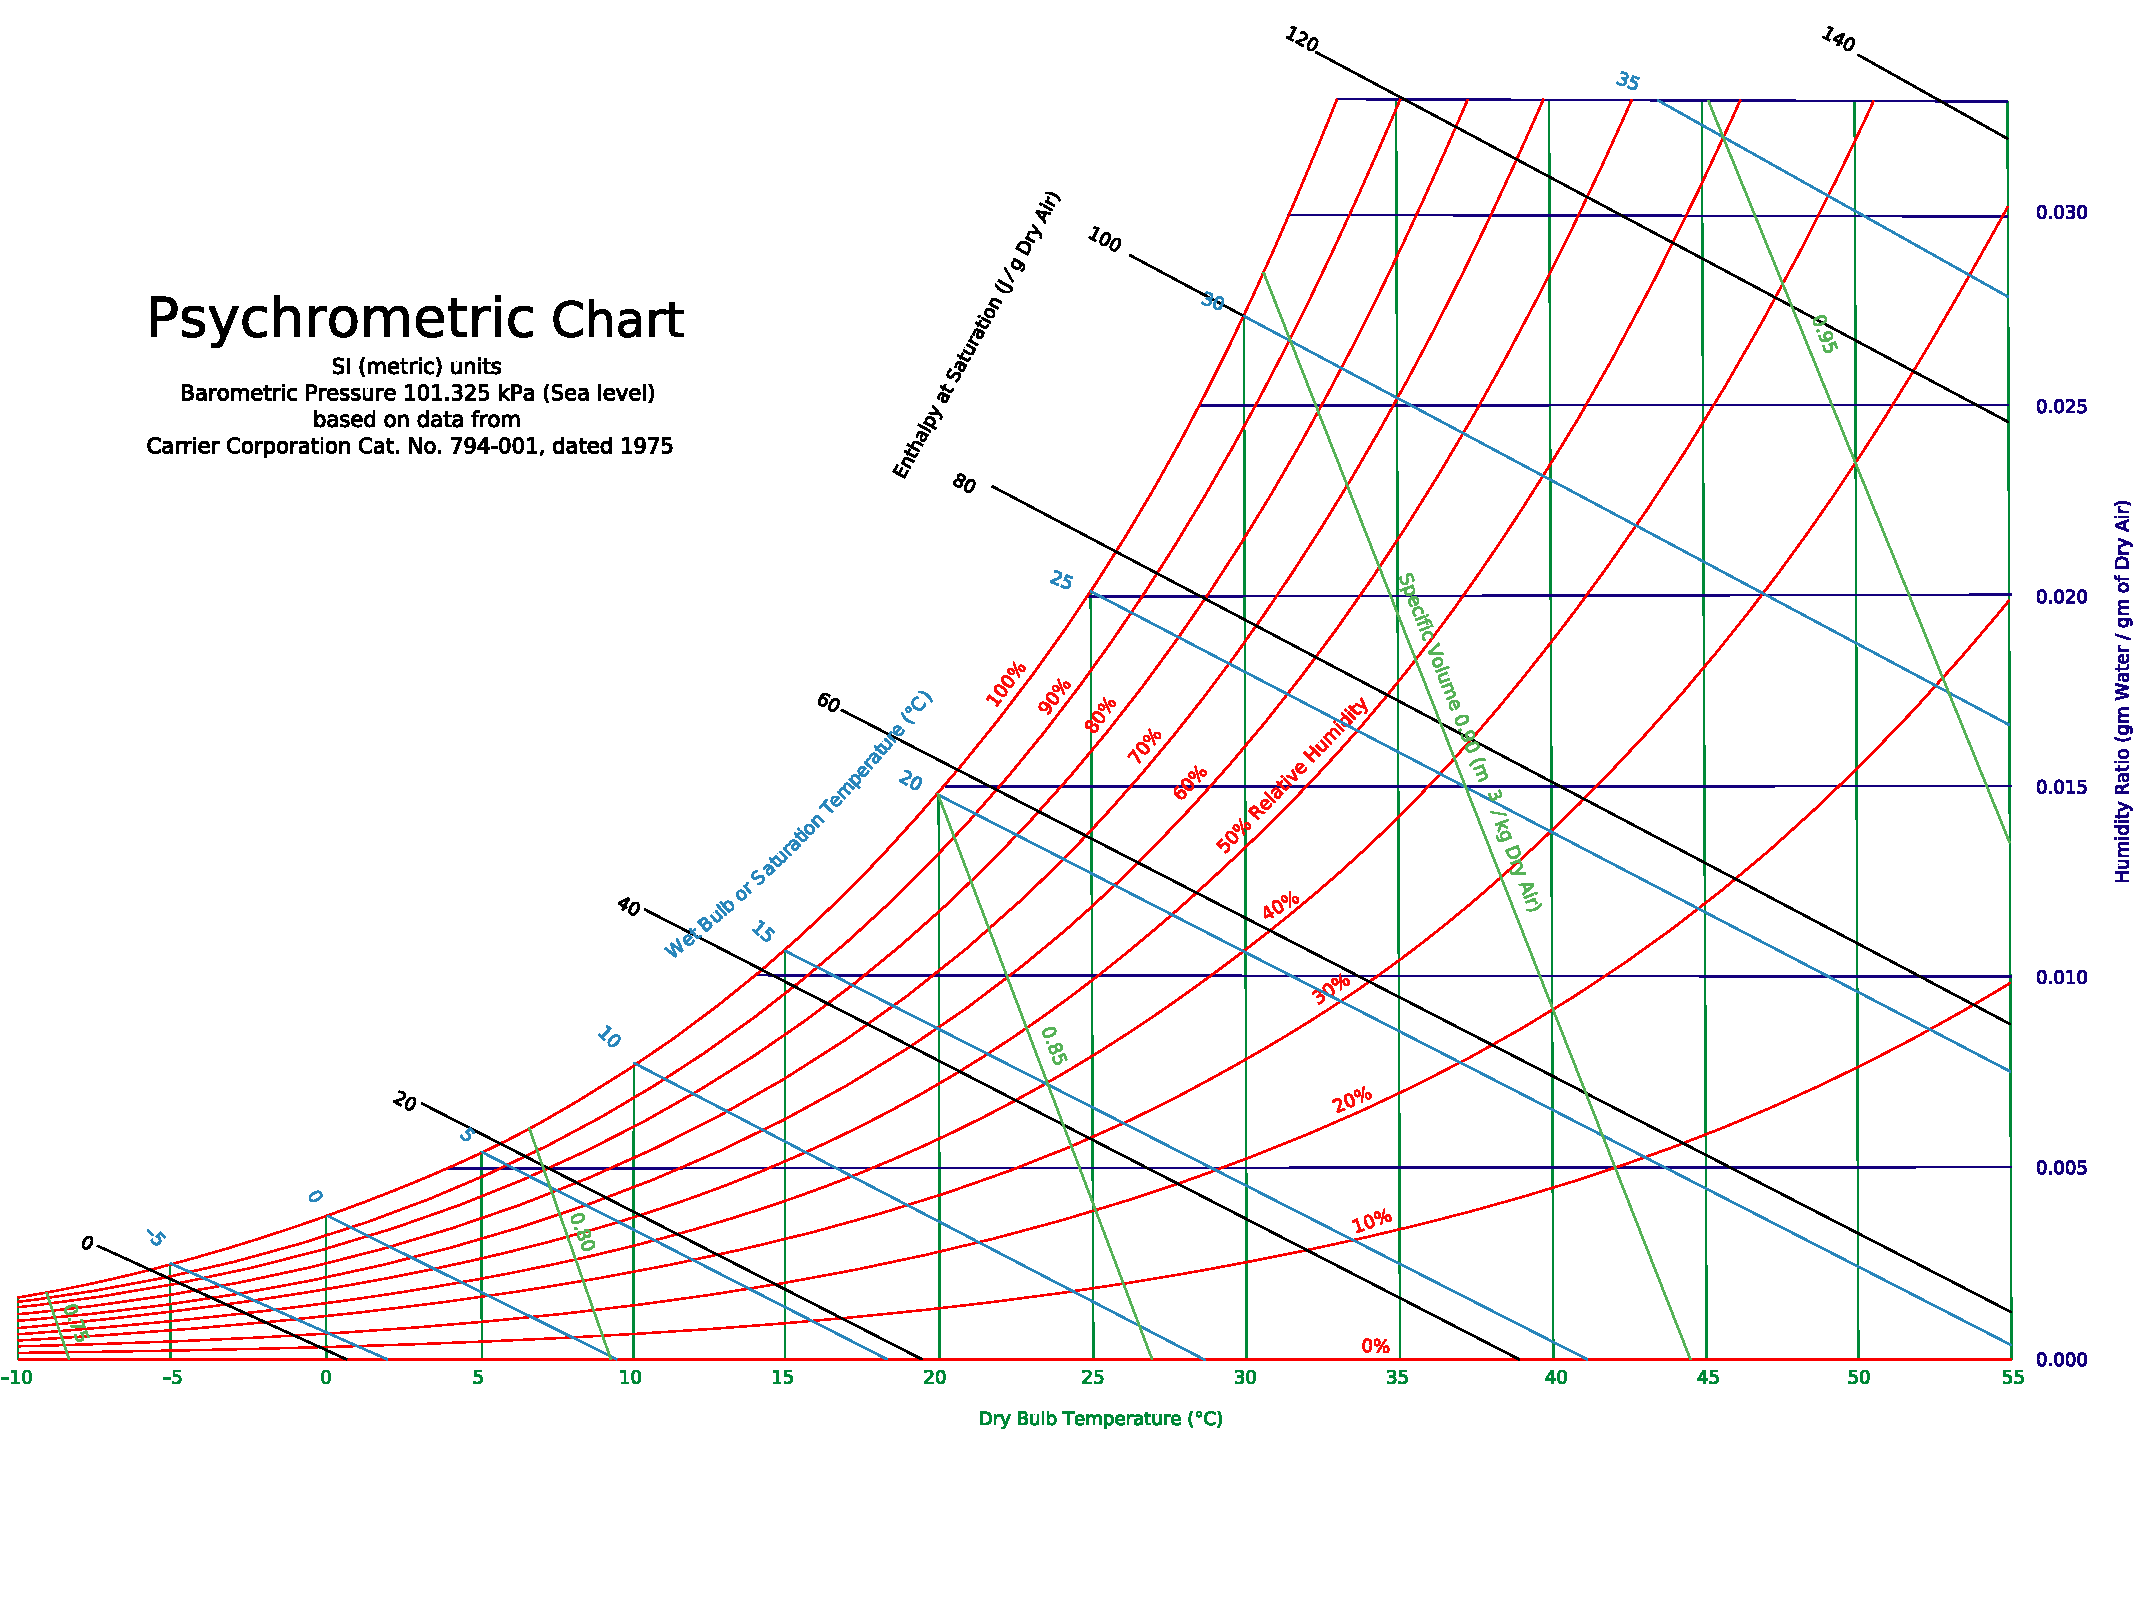
\includepdf[pages=-,fitpaper]{./Pics/PsychrometricChart}
  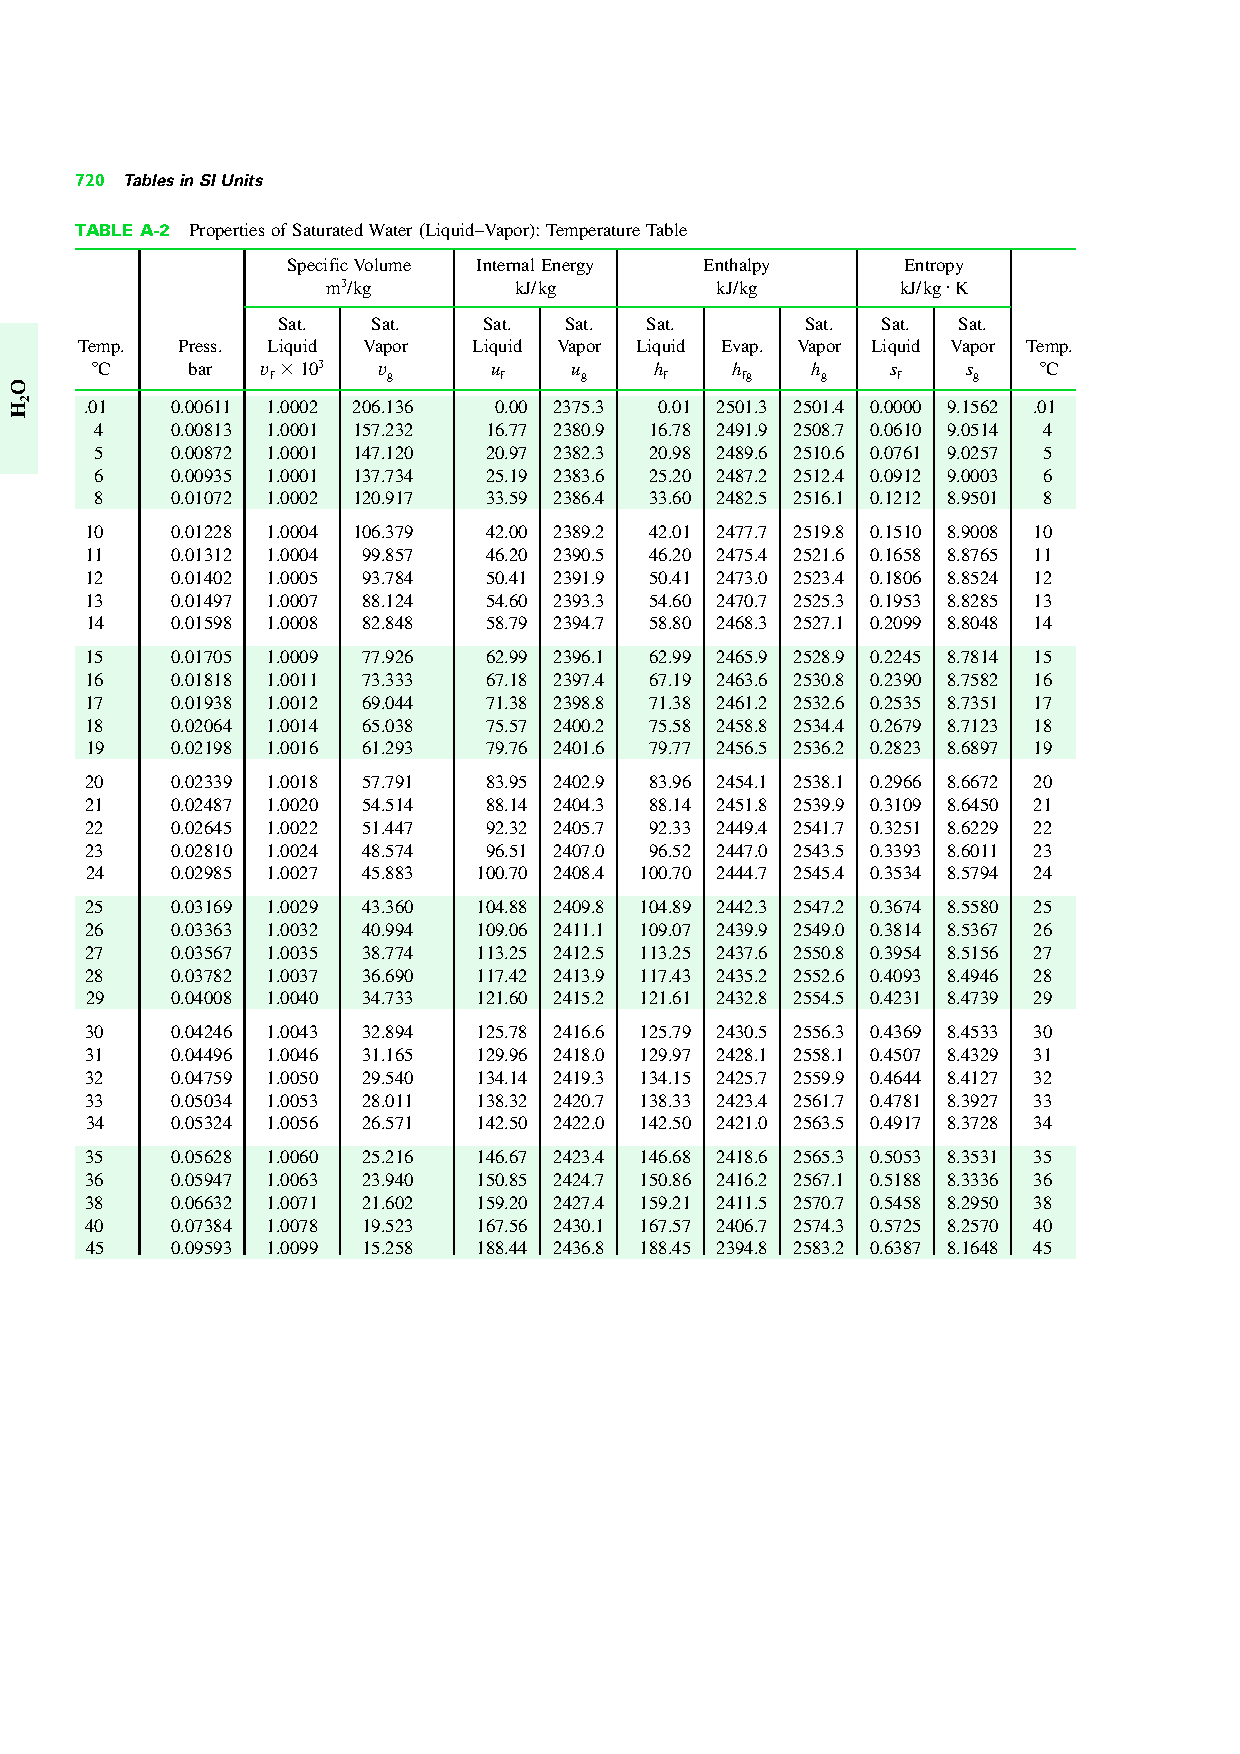
\includepdf[pages=-,fitpaper]{./Pics/H2O-R22_Table}
}
%\end{comment}

\end{document}
